\section{TODO}

\begin{enumerate}
    \item How to measure difficulty? Still an open question
    \begin{enumerate}
        \item Which agent is able to solve which datapoint?
        \item Compare "Breadth of expertise"
    \end{enumerate} [open]
    \item PSI vs In-house injections (compare std dev.) to support our in-house CWV score extractor. [Manaswi]
    \item "Developer Effort Mining Find GitHub repos with Lighthouse CI actions. Analyze PRs/commits that explicitly target CWV improvement (keyword search in commit messages: “lighthouse”, “performance”, “LCP”, “CLS”, “web vitals”). Measure: avg time to merge, number of iterations, lines changed. This gives a “developer effort” baseline without running a study." [Manaswi] 
    \item Qualitative Analysis of patches --> Show Patches alongside with Visual Changes as a figure. This is a strong point to show that non-trivial agent changes are required in some cases, to the reviewer. Also, show unsuccessful optimizations for ex. some lazy\_loading change that the agent made but failed. (Refer: https://arxiv.org/abs/2505.23671 : Fig. 7). 1st step --> Use LLM-as-a-judge to analyze b/w Agents. Also, think about: Reward Hacking + Regression. [Arnav] UPDATES --> (ran LLM-as-a-judge for the creation of a structured json schema for patch analysis --> made plots and tables on the insights --> need to spend a little more time on inferencing from these)
    \item Scatter plot for pareto rate vs dollars (Refer: TerminalBench, Screenshots on the group)[Arnav]
    \item Show if some agent struggles to improve some certain framework (use an LLM to analyze patches). 
    \item Budgetting using tokens analysis (reasoning): Only for Opencode: tbd when Agent runs are done i.e. will only do for a 2-3 agents.
    \item Tool calls: need to figure out how to fairly measure Agency of --> ClaudeCode (generally uses tons of toolcalls) vs OpenCode (moderate) vs Aider (very few). The purpose is to measure Agency.
\end{enumerate}

\subsection{E2E}
\subsubsection{Urgent: P0}
\begin{enumerate}
    \item Parallel Deploy + Bore + PSI [Manaswi, so everything except INP is working?] Initial, Final PSI scores + Commit ID? 
    \item Postprocessing [.env files, media,filter out .md files] [Somesh, Done, will use read/write only atm]
    \item Visual + DOM + Console errors validaition [Ayush]
    \item dot opencode config setup [Arnav] (Purpose: Reproducibility for 1. us to config another agent 2. someone else to reproduce [v1 Done for opencode]
\end{enumerate}

\subsubsection{Minor but Imp: P1}
\begin{enumerate}
    \item Data/Code release
    \begin{itemize}
        \item Rename to SWE-WEB
        \item Cleanup Repo w unnecessary files etc, Data columns
        \item Fix Readmes
    \end{itemize}
\end{enumerate}

\subsection{Arxiv/Neurips Todo}

\begin{enumerate}
    \item Impact: For a benchmark it should absolutely be clear that if an agent performs 83\% on our benchmark, what does it mean in absolute terms? e.g. SWE-Lancer earning an amount of dollars, SWE-Bench 70\% means it resolves 70 perc of real world issues, this is the most important point of our benchmark. The impact of our benchmark has three personas.
    \item Matching algorithm: If two websites share the backend/frontend tech stacks and have similar issues between our benchmark and actual websites.
    \begin{enumerate}
        \item 
    \end{enumerate}
    First filter the websites that share the tech stack distribution > X\%. Next, the issues identified by PSI should be common between matched website and real website. e.g. (00btweb.github.io -> bulk.com, they share 3 LCP and 2 CLS issues, good match). To measure the validity of matching algorithm, measure correlation of benchmark scores on AEM EDS/Headless with Benchmark.
    
    \begin{itemize}
        \item Web Users: By improving CWV we improve the web experience of the whole world look up the exact stats in this and \url{https://blog.chromium.org/2023/11/how-core-web-vitals-saved-users-10000.html} use current CrUX or internet traffic data to see that as of 2025 how much time e.g. 20,000 years of users do we show.
        \item Business: Case studies from deloitte etc, how many websites can we get to good scores and 100ms leading to improved outcomes etc
        \item Developer, How much developer productivity is improved, i.e. with what expertise and how many hours does it take for a CWV expeert or normal developer to fix a CWV issue: 1. For experts we will run human study with CWV experts at Adobe, for devs find repos with lighthouse installed somehow, either through gh api, static dataset (stack etc), dataset of commits (figure out), then find PRs/commits that explicitly aim to solve CWVs through commit messages and diffs, then find the avg number of hours or tries (through prev commits to solve these issues)
    \end{itemize}
    \item Data Contamination: Our pitch would now be that we are contamination resistant, because we have a verifiable reward metric and automated data curation pipeline as opposed to static dataset. So whenever a model is released we can test it X weeks later in terms of absolute and arena rankings, and by these X weeks we will have enough points to evaluate models. Further we will maintain an Adobe internal enterprise benchmark similar to SWE-Bench Pro, making a held out set. I can make the new data points from entirely new repos/commits which we will decide experimentally.
    \item Positioning of our benchmark: Here we have to define the scope of problem statement that our benchmark evaluates, how good of a benchmark it is in those terms. We measure webpage optimization, first we have to prove its relevance and importance, through Impact, and through Industry we need numbers through crux or developers or business that actually need this. Next, since this is narrow scope of webpage optimization we have to prove that what breadth of real world capabilities does our dataset measure, this is the hardest question to answer so far.
    \begin{itemize}
        \item We have to show its not surface level frontend debugging and not just that these problems are difficult, but they require a wide domain of webpage expertise, both from some literature \url{https://arxiv.org/html/2412.07892v1} and analysis of our dataset
        \item The problems, solutions, and data points in our benchmark are diverse, and because its a live/evolving bench, it measures longitudnal capabilities both past and cutting edge tech.
    \end{itemize}
    \item Preliminary technical questions and how do we tackle them?
    \begin{itemize}
    \item Do metrics on our benchmark really correlate with the real world outcome? Prove it, we have to solve them through assuming AEM EDS to be the distribution of real world popular websites, we have to solve these challenges ``Is the distribution of SWE-WEB and real world websites similar" in terms of [Arnav/Ayush]
    \begin{itemize}
        \item Users: Off the bat, no, because public github websites are not the same as real world websites. But how similar? How faithfully do evaluations translate from our benchmark to real world websites? Correlation btw perf on SWE-WEB and SWE-WEB Adobe Enterprise. This aligns distribution of our benchmark to real world business websites which have the real world traffic.
        \item In terms of tech: How well do websites in our benchmark correlate to real world websites in terms of the tech stacks and complexity? The frameworks they use, the size of the repos etc how well aligned are they aligned
        \item Technically our metrics are Pareto rate, Site health etc, are the set of them complete and non redudnant in measuring optimization? what do they individually mean
    \end{itemize}
    \item How resistant is our benchmark really? [Manaswi]
    \begin{itemize}
        \item How many new datapoints can I make, how long do I have to wait to make the benchmark work after a training cutoff date?
        \item How much data contamination is evaded if I do RL on previous commits / repos from this distribution? 
        \item Commit vs Repo? are K-commits of distance enough or do we need entirely new repos?
    \end{itemize}
    \item How sound is our benchmark?
    \begin{itemize}
        \item Visual Regression, show qunatitative and qualitative examples of Vis Regresisons [Ayush]
    \end{itemize}
    \item Experiments, Analysis, and Insights of our paper    
        \item Run on more agents, add open source [Arnav + Somes]
        \item What is the effect of agent vs LLMs, trajectory metrics or LLM or agent capabilities, how do we deconfound or analyze these?
    \end{itemize}
\end{enumerate}




\subsection{P1}
\begin{enumerate}
    \item Run framework identification on 7389 and check no stack is missing
\end{enumerate}

\subsection{CWV Agent v2 [Wed]}

\begin{enumerate}
    \item cwv-agent v2 (production) + opencode/claudecode (research) 

    \item CWV Measurement
    \begin{itemize}
        \item Cloudflared + PSI Script [Arnav] \arnav{Cloudflare rate limits after 15 calls.}
        \item ngrok (auth)
        \item Avg time and rate limit for PSI \arnav{Avg. PSI time = 20s per/PSI report}
        \item discuss bottlenecks on CPU/LLM (coding agents) on subset of 300, external deployment
    \end{itemize}
    \item CWV Agent v2
    \begin{itemize}
        \item Rate Limit
        \item Context Length errors \arnav{Caused due to large PSI reports containing page asset details.}
        % \item The average time, average number of suggestions [Arnav]
        % \item What is causing these context bloats? [Arnav: 10]
        % \item What is the average time taken otherwise? [Arnav: 10]
        % \item What to remove from PSI [Arnav:10]
    \end{itemize}    
    \item Coding Agent: Why is it taking 180 s per suggestion (avg:4)
    \item Fix the CWV measurement after optimization
    
    \item Send the total run scores [Arnav] \\
     ((GPT5, Gemini), (GPT5, Gemini, Claude Sonnet 4.5)) \\
     ngrok / cloudfare tunnel then use PSI to measure CWV scores on this hybrid deployment
     \arnav{Suggestions taking over a day for 30 samples. Full pipeline is working: \\2 bottlenecks: \\1. agent inference latency due to an average of \~4 suggestions per datapoint \\2. Context length error due to un-shortened PSI Reports being inputted.}
    \item Eval scripts + Refresh of the scores [Somesh]
    \item EDS benchmarking get reviewed by Julien [Somesh,Ayush:10]
    \begin{itemize}
        \item Customer source codes at \url{https://github.com/orgs/aemsites/repositories} and \url{https://github.com/hlxsites/} Check with Julien, which ones are customer repos
        \item Setting up instructions: \url{https://www.aem.live/developer/tutorial\#start-developing-styling-and-functionality} + local instructions
    \end{itemize}
    \item EDS benchmarking extend to customers [Ayush]
    \item Content similarity [Ayush, Wed]
    \item Use Adobe PSI [Arnav]
    \item Cloudflare + PSI [Arnav]
\end{enumerate}
\subsection{ASO Alignment}
\begin{enumerate}
    \item LLM pipeline for identifying tech stack, send results + review, distribution, script push [Manaswi + Somesh,10pm]
    \item Run wappalyzer on SWE-WEB, push to HF [Manaswi]
    \item Get list of domains for ASO headless Customers [Somesh] \somesh{Done for 300/427 and sent, remaining are processing slowly}
    \item EDS Static + CrUX Benchmark [Ayush] 
    \begin{itemize}
        \item EDS (filter EDS with Code level check)
        \item check correlation between just file extension .bundle/.min vs code fetching
    \end{itemize}
    \item Identify static websites from Github (not github .io) [Manaswi]
\end{enumerate}

\subsection{Current benchmark}
\begin{enumerate}
    \item Do the full run for CWV -- dependent on whether we decide to use PSI or not [Arnav]\\
    \arnav{I need the 2nd machine for this...} [Somesh]\\
    Push the updated CWV Extraction code [Arnav] [Done]
    \item Internal PSI [Somesh] \somesh{Pushed the code to git, need to check on CPU machines and rate limit discussion + local hosting}
    \item Playwright Lighthouse [Somesh, Closed]
    \item Debug Claude Code + Claude Models [Arnav] [Done]\\ \arnav{log analysis: "**Estimated total effort:** 40-50 hours over 4 weeks
**Expected ROI:** 15-25\% improvement in conversion rates, 10-20\% reduction in bounce rates"}
    \\
    Run GPT5.1 Codex on the same input. [Arnav] [Done]
    \item Push the Eval Code (Pareto, Health, $\Delta$ etc.) [Somesh]
    \item Look at existing literature (from a SWE perspective) that compares CWV extraction methods
    \item CWV Evaluation is slow [Somesh]
    \begin{enumerate}
        \item Parallelize the agent benchmarking by [Arnav] [More or less Done] [Push to a new branch]
        \begin{enumerate}
            \item Generating N patches
            \item Instead of git clone: Apply on the repo and evaluate parallely
        \end{enumerate}
        \item Add Visual Validation at the end of the agent benchmarking [Arnav] [Done]
        \item Improve parallelization [Arnav] [Done]\\
        \arnav{Current stats: 9.6mins for 30 datapoints with 5 runs each $\implies$ 4s per run}
        \arnav{Open a PR for cwv\_benchmark.py [Done]}
        \item Deprioritize LCP, Read Correlation of LCP / CLS / INP (read crux research) [Somesh]
        \item What is Average LCP time vs INP/CLS [Arnav]? --> Use hybrid Network Simulation (initially fast, then make it slow)
        \item Check CWV implementation with AEM [Somesh]
        \item What is the effect of reducing number of runs
        \begin{itemize}
            \item Try on github live compare to EDS to check if major variance is due to network 
        \item Get current implementation reviewed
        \end{itemize}
    \end{enumerate}
    \item Add Webpage Type [Ayush] (Screenshot + model, Title/Meta)
    \begin{itemize}
        \item 12 classes [Ayush]
    \end{itemize}
    \item Improve Budget (Time/Cost/Tokens/Calls etc)  [Somesh]
    \item Evaluating Agency [Somesh]
    \item Dockerization [Ayush]
    \item Update Instructions [Somesh]
    \item Extend Stacks [Manaswi]
    % \item Try prompt optimization 
    % \item Prompt optimization for claude (using GEPA, give actual INP / CLS elements)
    \item Add Open Source [Somesh]
    \item Add Gemini [Somesh]
\end{enumerate}

\subsection{Next Steps}
\begin{enumerate}
    \item Lighthouse GH Action history (how to get history) PR's dataset + (only work for PR not commit) [Ayush: \somesh{Use .github/workflows.y*ml}]
    \begin{itemize}
        \item github.io -> .github/workflows.yml .yaml
        \item Whole stack -> lighthouse action
    \end{itemize}
    \item A short demo video, YT Creds [Yaman]
    \item MCP Tool for CWV
    \item Extending Data from Tranco non-minified [Ayush]
    \begin{itemize}
        \item How much do patches transfer, allowing us horizontal scale
    \end{itemize}
    \item Extending Data from Commits
    \begin{itemize}
        \item There might be deployment errors and Tech Stack might change
        \item Ensuring Webpage Content does not change substantially in terms of Performance
        \item Create Natural Code Experiments for Performance
    \end{itemize}
        \item Website


\end{enumerate}

\section{Discussions}
\begin{itemize}
    \item Convert datapoints into easy / medium / hard.
    \item How to align it to closer real world economy? Expert effort? Dev effort?
    \item Evaluating Agency [Somesh]
    % Arnav: Run 1- Input: Poor Mobile CWV scores; LLM is able to fix. Run 2- Input: Same Poor Mobile CWV scores as well as Strong Desktop CWV scores; LLM isn't able to make the same amount of improvement in Mobile CWV whilst maintaining Desktop CWV.
    \somesh{Interesting data source https://ghtorrent.github.io/tutorial/}
    \item SWE-Bench-Verified vs SWE-Bench-Pro (https://openai.com/index/why-we-no-longer-evaluate-swe-bench-verified/):
    \begin{enumerate}
        \item Too narrow and too wide tests
        \item Data leaks / contamination: For this, we should try and do qualitative analysis on the datapoints that all Agents can solve (analyse their patches etc.). 
        \item We should emphasize that our reward function / scoring is practically perfect, as it is quantitative and doesn't involve situations like incomplete unit tests or such.
        \item \textbf{Need to build some sort of anti-contamination pipeline}
    \end{enumerate}
\end{itemize}
    
\paragraph{Dataset Schema: UPDATE}
Our Dataset
ID, Github Username/Reponame, Tech Stack Commit ID, ZIPped Repository Path, (host.sh), {Desktop LCP, Desktop CLS, Desktop FID, Desktop INP, Desktop TTFB, Mobile LCP, Mobile CLS, Mobile FID, Mobile INP, Mobile TTFB}

\section{Comments}

\arnav{Arnav:
\begin{itemize}
    \item Add appendix listings for \textit{everything}.
    \begin{enumerate}
        \item LCP, CLS, INP: measurement and elements extraction using js injections.
    \end{enumerate}
    \item Mention that LCP(p75), INP(p75), CLS(median) are ADOBE standard conventions, in the paper text. 
    \item Ensure console logs are foolproof
    \item{Decide whether to keep Manual Heuristic Filtering or completely automate it or even do a hybrid}
    \item Get correlation scores b/w runs=30, runs=15 and runs=5 for cwv\_benchmark
    \item Validate and log (make a table of) all the simulated clicks on a webpage
    % \item Extract INP, CLS elements as well [DONE]
    \item Comparisons b/w tech stacks: Do EDA of CWV (before and after) vs tech stack, then infer and decide what to keep and what not to 
    \item Tag datapoints as Easy/Medium/Hard - on what basis?
    \item Extend tool calls and log them for consistency across agents
    \item Fine-tune on train split datapoints (look for appropriate methods in lit., GRPO etc)
\end{itemize}
}

\manaswi{
\begin{enumerate}
    \item Fix framework identification heuristic + automatic
    Check all framework identifications seperately -> Checked for react, seperate from next.js (causing a huge chunk to be lost)
    Find old code to use and build upon -> cant find at all :(
    \item LLM pipeline for visual recognition
    cant find any pre-exisitng mechanisms doing simply visual recgonition, there is recognintion of third party apps like payement interfaces and cookie permissions. Found exisitng work of Builtwith and Whatruns but all are closed private agents. 
\end{enumerate}
}

%% ================================================================
\subsection{Core Thesis (1 sentence)}
%% ================================================================
\OurBench is the first benchmark that evaluates coding agents on improving \emph{real user experience}---bridging the gap between code-generation metrics and measurable real-world impact by targeting Core Web Vitals on deployed websites, making it simultaneously \textbf{impact-aligned}, \textbf{contamination-resistant}, and a \textbf{long-horizon autonomy probe}.

%% ================================================================
\subsection{Three Pillars of Differentiation}
%% ================================================================

\subsection{Refined Contribution List (for Introduction)}
%% ================================================================

\begin{enumerate}
    \item \textbf{Benchmark + Dataset.} We introduce \OurBench, the first execution-based benchmark evaluating autonomous coding agents on user-facing web performance optimization. The benchmark spans 2,741 repositories and 73,000 deduplicated webpages across 11 frameworks (React, Vue, Next.js, Hugo, Jekyll, Hexo, etc.) covering 70\% of GitHub Pages web stacks---the largest web-focused coding agent benchmark to date, and the first to target JavaScript/TypeScript-dominant codebases at scale.

    \item \textbf{Impact-Aligned Evaluation Harness.} We design a containerized, framework-agnostic harness that measures Core Web Vitals via Playwright instrumentation, achieving Spearman $\rho = 0.87$ with real-world CrUX field data. The harness enforces visual, DOM, content, and console-error regression checks, preventing reward hacking while providing a continuous optimization signal suitable for both evaluation and RLVR-based agent training.

    \item \textbf{Contamination-Resistant Architecture.} Unlike static patch-matching benchmarks, \OurBench defines success through dynamic runtime measurement of deployed webpages, making memorization ineffective. We demonstrate a continuous benchmark refresh pipeline via the GH-25 corpus and validate contamination resistance through temporal and commit-distance analyses.

    \item \textbf{Systematic Evaluation Revealing Capability Gaps.} We evaluate 4 agents $\times$ 4 frontier LLMs, finding:
    \begin{itemize}
        \item Best configuration (OpenCode + GPT-5.1 Codex) achieves 57\% Pareto improvement rate; worst (GPT-4.1) degrades 90\% of sites.
        \item Vanilla prompting yields 0\% improvement with any model---structured plan-then-implement protocol is necessary.
        \item Agent scaffold governs multi-metric planning (16$\times$ gap at fixed model); LLM capability governs regression avoidance.
        \item Surgical precision (9 \texttt{defer} attributes) predicts success; broad rewrites (34 files, 116 preload directives) predict failure.
        \item No agent achieves a calibrated ``do nothing'' policy for already-optimal sites.
    \end{itemize}
\end{enumerate}

%% ================================================================
\subsection{Anticipated Reviewer Questions \& Preemptive Defenses}

\subsubsection{Q1: ``Isn't this just frontend debugging? How hard/diverse is web performance optimization?''}
\textbf{Defense:}
\begin{itemize}
    \item \textbf{Empirical difficulty:} Best agent achieves only 57\% Pareto rate. Vanilla prompting: 0\%. GPT-4.1 degrades 90\% of sites. This is harder than SWE-Bench Verified (72\%+ for frontier models).
    \item \textbf{Breadth of expertise required:} CWV optimization spans: resource loading strategy (preload/prefetch/defer), CSS critical path optimization, image format selection and lazy loading, JavaScript execution optimization, font subsetting, DOM structure, caching strategy, code splitting, third-party script management, layout stability engineering. Reference: web.dev optimization guides catalog 50+ distinct optimization techniques. \somesh{cite from https://arxiv.org/html/2412.07892v1}
    \item \textbf{11 frameworks:} Each framework has different build pipelines, asset handling, and optimization surfaces. Static HTML vs React vs Next.js require fundamentally different approaches.
    \item \textbf{Multi-objective complexity:} Optimizing LCP can degrade CLS (our data shows this concretely). No single-objective benchmark captures this.
    \item \textbf{Add experiment:} Categorize the 300 evaluation websites by difficulty (baseline CWV tiers) and required optimization type. Show distribution across at least 10 distinct optimization categories. \somesh{Similar to CodeClash etc where issue/solution types are resolved via LLM as a judge}
\end{itemize}

\subsubsection{Q2: ``Static sites on GitHub Pages are too simple. Does this generalize to real-world production websites?''}
\textbf{Defense:}
\begin{itemize}
    \item \textbf{CrUX correlation:} $\rho = 0.87$ with real-world field data. The relative performance ordering of sites in our harness mirrors production traffic conditions.
    \item \textbf{Complexity stats:} Median 334 files, p90 2,718 files. Median 121K LoC, p90 1.08M LoC. These are not toy repos.
    \item \textbf{Framework coverage:} 11 frameworks covering 70\% of GitHub Pages stacks. React, Vue, Next.js are production-grade frameworks.
    \item \textbf{Enterprise validation:} [If available] Show correlation between agent performance on \OurBench vs. Adobe AEM/EDS enterprise websites. Even directional evidence (e.g., same rank ordering) would be powerful.
    \item \textbf{Cite precedent:} SWE-Bench uses only 12 Python repos. SWE-Lancer uses a single Expensify repo. Our 2,741 repos is orders of magnitude more diverse.
    \item \textbf{Static sites ARE the web:} GitHub Pages hosts millions of sites. CWV issues are frontend-bound---the same bottlenecks (render-blocking resources, layout instability, unoptimized images) affect both static and dynamic sites.
\end{itemize}

\subsubsection{Q3: ``How do you know your lab CWV measurements are reliable? CWVs are notoriously noisy.''}
\textbf{Defense:}
\begin{itemize}
    \item \textbf{30 runs per (site, device):} Fresh browser context each run, IQR-based outlier removal, p75 aggregation consistent with Google/Adobe conventions.
    \item \textbf{CrUX validation:} $\rho = 0.87$ Spearman rank correlation with field data. This is strong evidence of measurement fidelity.
    \item \textbf{Noise calibration:} Table~\ref{tab:thresholds-full} reports empirically calibrated noise tolerances (e.g., LCP Mobile: 100ms noise tolerance, 200ms meaningful improvement threshold = 2$\times$ noise floor).
    \item \textbf{Containerized environment:} Standardized Docker, CPU throttling, network shaping eliminate environmental variance.
    \item \textbf{Add experiment:} Report test-retest reliability: measure the same site twice on different days, compute ICC (intraclass correlation). Target: ICC $> 0.9$. [Somesh]
\end{itemize}

\subsubsection{Q4: ``Can agents hack the evaluation by removing content, hiding elements, or breaking functionality?''}
\textbf{Defense:}
\begin{itemize}
    \item \textbf{Four-layer regression checks:} (i) GPT-4.1 visual similarity, (ii) DOM LSH consistency, (iii) Jaccard content similarity $\geq 0.97$, (iv) No new console errors.
    \item \textbf{Build failure = invalid:} Any deployment failure invalidates the attempt.
    \item \textbf{Concrete evidence:} Show examples where regression checks caught reward hacking attempts. E.g., agent removed images to improve LCP $\rightarrow$ caught by visual regression. Agent disabled JavaScript $\rightarrow$ caught by console error check.
    \item \textbf{Comparison:} SWE-Lancer Appendix A7 shows unit tests are hackable (variable renaming bypasses check). Our E2E visual+DOM+content checks are structurally harder to exploit.
\end{itemize}

\subsubsection{Q5: ``Why not use PageSpeed Insights (PSI) or Lighthouse instead of custom Playwright injection?''}
\textbf{Defense:}
\begin{itemize}
    \item \textbf{Lighthouse is lab-only:} Does not measure INP (requires real interaction). Our harness simulates real user interactions (scroll, click, type).
    \item \textbf{CrUX correlation validates our approach:} $\rho = 0.87$ shows our custom measurement is faithful to real-world metrics.
\end{itemize}

\subsubsection{Q6: ``You only test 4 agents and 4 LLMs. Is this comprehensive enough?''}
\textbf{Defense:}
\begin{itemize}
    \item \textbf{Ablation design:} Our 6 configurations enable clean agent-vs-LLM disentanglement. This is methodologically stronger than testing 20 models without ablations (as many benchmarks do).
    \item \textbf{Precedent:} SWE-Bench original tested 5 models. AlphaCode tested 1 system. SWE-Lancer tested 3 models.
    \item \textbf{Key finding is robust:} The 16$\times$ agent scaffold gap and the surgical-vs-broad-rewrite pattern are consistent across all configurations.
    \item \textbf{Add:} Open-source models (Qwen3-Coder, DeepSeek-V3, Kimi K2) via OpenCode. At least 2-3 open models to show the gap. [Arnav + Somesh]
    \item \textbf{Add:} Gemini 2.5 Pro or Gemini 3 Pro for Google model coverage. [Somesh]
\end{itemize}

\subsubsection{Q7: ``No human baseline. How do we calibrate what 57\% Pareto rate means?''}
\textbf{Defense (CRITICAL --- this is the biggest gap):}
\begin{itemize}
    \item \textbf{Option A: Expert study.} Run CWV experts at Adobe on 20-30 sites. Measure time, success rate, optimization strategies. This provides calibration: ``Experts achieve X\% in Y hours; best agent achieves 57\% in 15 minutes.'' [Somesh --- HIGH PRIORITY]
    \item \textbf{Option B: Developer effort mining.} Find GitHub repos with Lighthouse CI actions. Analyze PRs/commits that explicitly target CWV improvement (keyword search in commit messages: ``lighthouse'', ``performance'', ``LCP'', ``CLS'', ``web vitals''). Measure: avg time to merge, number of iterations, lines changed. This gives a ``developer effort'' baseline without running a study.
    \item \textbf{Option C: Economic calibration.} Map Pareto rate to CWV tier transitions. ``57\% Pareto rate = 0.93 net threshold crossings per site = X websites moved from Poor to Good. At Deloitte's 10\% conversion rate per 0.1s LCP improvement, this corresponds to Y\% revenue uplift across the benchmark.''
    \item \textbf{All three should be pursued.} Option C is cheapest and can be done now. Option B requires data mining. Option A requires coordination with Adobe.
\end{itemize}

\subsubsection{Q8: ``Your benchmark is web-specific. Isn't this too narrow for a top venue?''}
\textbf{Defense:}
\begin{itemize}
    \item \textbf{Web development is the largest SE domain:} 50\% of developers, 40\% of revenue, yet 0\% of SWE-Bench/BigCodeBench/LiveCodeBench coverage. \somesh{Bring exact figures for this statement and cite it}
    \item \textbf{CWV optimization is a microcosm of real SE:} Diagnosis, multi-file changes, regression prevention, performance profiling, iterative refinement. It requires the same skills as general performance engineering. \somesh{We need to make sure with high precision that this point is enough by comparing relative difficylty, because other benchmarks also achieve this, rather leverage like these are actual issues/bugs that are poisoning the web experience today, example of this can be seen in https://arxiv.org/html/2412.07892v1}
    \item \textbf{Precedent for domain-specific benchmarks at top venues:} SWE-Lancer (single Expensify repo), AlphaCode (competitive programming only), SWE-fficiency (runtime optimization only). Each fills a specific evaluation gap. \somesh{This is not the ideal way, we should make it implicit, not rely}
    \item \textbf{Breadth within the domain:} 11 frameworks, 2,741 repos, 73K webpages. This is not narrow---it's the broadest web-focused evaluation by orders of magnitude.
    \item \textbf{RLVR implications are general:} The continuous-reward, contamination-resistant structure applies beyond web optimization. Our design pattern (dynamic measurement + automated environment) is a template for other domains. \somesh{Ignore this point unless we actually show results on Web-Opt}
\end{itemize}

\subsubsection{Q9: ``How is this different from SWE-fficiency which also measures performance?''}
\textbf{Defense:} \somesh{This whole point has to be conveyed implicitly, in terms of impact alignment and user facing metrics + importance, scale, time evolving, avoid over comparison}
\begin{itemize}
    \item \textbf{User-facing vs. developer-facing:} SWE-fficiency measures runtime speedup (developer concern). We measure CWVs (user experience concern $\rightarrow$ economic impact $\rightarrow$ search ranking).
    \item \textbf{Multi-objective:} SWE-fficiency has a single objective (speedup). We have 6 interacting metrics.
    \item \textbf{Field validation:} SWE-fficiency has no field validation. We have $\rho = 0.87$ with CrUX.
    \item \textbf{Anti-reward-hacking:} SWE-fficiency relies on unit tests for correctness. We have visual+DOM+content+console checks.
    \item \textbf{Scale:} SWE-fficiency: 498 tasks from 9 Python repos. \OurBench: 73K webpages from 2,741 repos across 11 frameworks.
    \item \textbf{Language:} SWE-fficiency: Python. \OurBench: JS/TS/HTML/CSS (the most underrepresented domain).
\end{itemize}

\subsubsection{Q11: ``CLS and INP barely improve. Are they measurable in your harness?''}\somesh{@Arnav CLS/INP inputs}
\textbf{Defense:}
\begin{itemize}
    \item \textbf{They ARE measurable:} Our harness detects CLS/INP regressions precisely (Claude Code causes CLS 0.094 $\rightarrow$ 1.08; Aider causes INP 16ms $\rightarrow$ 752ms). The harness is sensitive enough to detect both improvements and degradations.
    \item \textbf{Difficulty is the finding:} CLS/INP are harder to optimize than LCP because they require understanding of user interaction patterns and layout stability, not just resource loading. This is a genuine insight about model capabilities.
    \item \textbf{Add experiment:} Per-metric success rate breakdown. Show that LCP improves in X\% of cases, CLS in Y\%, INP in Z\%. Identify which metric is the primary bottleneck for each failure mode. [Arnav]
\end{itemize}

%% ================================================================
\subsection{Experiments, Analysis, and Figures to Add (Priority Ordered)}
%% ================================================================

\subsubsection{P0: Must-Have for Submission}

\begin{enumerate}
    \item \textbf{[TABLE] Benchmark Comparison Table.} Side-by-side comparison of \OurBench vs SWE-Bench, SWE-Lancer, LiveCodeBench, BigCodeBench, SWE-fficiency, Terminal-Bench. Dimensions: Language, Scale, Metric Type, Contamination Defense, Field Validation, Multi-Objective, RLVR-Ready. \textit{This is the single most important table for positioning.} [Somesh]

    \item \textbf{[EXPERIMENT] Open-Source Models.} Run at least 2-3 open models (Qwen3-Coder, DeepSeek-V3, Kimi K2) via OpenCode. This addresses reviewer concern about frontier-only evaluation and reveals the open-vs-closed gap. [Arnav + Somesh]

    \item \textbf{[EXPERIMENT] Difficulty Stratification.} Categorize 300 eval websites into Easy/Medium/Hard based on baseline CWV profile. Report Pareto rate per difficulty tier per agent. \textit{Inspired by Terminal-Bench's difficulty analysis and AlphaCode's rating-bucket breakdown.} [Arnav]

    \item \textbf{[ANALYSIS] Economic Impact Quantification.} Map Pareto rate $\rightarrow$ CWV tier transitions $\rightarrow$ business impact. ``57\% Pareto rate on 300 sites = N sites moved from Poor$\rightarrow$Good. Using Deloitte's conversion data, this corresponds to X\% revenue uplift per site.'' Include CrUX data on how many real-world origins have Poor CWVs. [Somesh]\somesh{We dont have impact precednts directly as of now good for arxiv}

    \item \textbf{[TABLE] Per-Framework Agent Performance.} Heatmap or table: rows = agents, columns = frameworks (Static HTML, Jekyll, Hugo, Hexo, React, Vue, Next.js). Cells = Pareto rate. \textit{Shows whether certain frameworks are harder and whether agents specialize.} Inspired by BigCodeBench's domain specialization analysis. [Arnav]\somesh{Need t decide for better presentation this isnt good enough}
\end{enumerate}

\subsubsection{P1: High-Value Additions}

\begin{enumerate}
    \item \textbf{[EXPERIMENT] Human Expert Baseline.} 20-30 sites evaluated by CWV experts at Adobe. Measures: success rate, time, optimization strategies, lines changed. This provides the human calibration that SWE-Lancer and AlphaCode both use effectively. [Somesh --- coordinate with Adobe]

    \item \textbf{[EXPERIMENT] Contamination Resistance Validation.}
    \begin{itemize}
        \item Temporal analysis: Stack (older) vs GH-25 (newer) performance comparison.
        \item Fine-tuning experiment: Fine-tune on benchmark repos, show no CWV optimization improvement.
    \end{itemize}
    [Manaswi]

    \item \textbf{[FIGURE] Pareto Frontier Visualization.} Scatter plot: x-axis = \% sites improved, y-axis = \% sites degraded. Each point = one agent configuration. Ideal = top-left corner. \textit{Inspired by Terminal-Bench's cost-performance Pareto.} [Ayush]

    \item \textbf{[FIGURE] Per-Metric Improvement Distributions.} Violin/box plots showing the distribution of LCP, CLS, INP changes across all 300 sites for each agent. \textit{Shows not just means but the full distribution of outcomes.} [Arnav]

    \item \textbf{[ANALYSIS] Optimization Strategy Taxonomy.} Classify all agent patches into optimization categories (defer scripts, preload LCP image, compress images, inline critical CSS, lazy load, code split, etc.). Report frequency and success rate per category per agent. \textit{Inspired by SWE-fficiency's profiling-based attribution and AlphaCode's problem-type breakdown.} [Arnav/Somesh]

    \item \textbf{[EXPERIMENT] Budget/Scaling Analysis.} Run the best agent with 5/10/15/25 interaction steps and 5/10/15 minute time limits. Plot Pareto rate vs budget. \textit{Answers: ``Would more budget solve the problem?'' Inspired by AlphaCode's sample-count scaling and Terminal-Bench's compute analysis.} [Arnav]

    \item \textbf{[EXPERIMENT] Cross-Benchmark Correlation.} For the 4 LLMs tested, plot their \OurBench Pareto rate vs their SWE-Bench Verified score. If correlation is low, this proves \OurBench measures something different. If high, it validates alignment. Either outcome is publishable. [Somesh]

    \item \textbf{[FIGURE] Failure Mode Gallery.} 2$\times$3 grid of before/after screenshots showing: (a) successful optimization (visually identical, better CWVs), (b) CLS regression (FOUC), (c) broken page (404 errors from non-existent files), (d) content removal caught by regression check. \textit{This is the most intuitive way to communicate what the benchmark evaluates.} [Ayush]

    \item \textbf{[TABLE] Trajectory/Behavior Statistics.} Per agent: avg turns, avg tokens consumed, avg time, avg tool calls, file read/write ratio, web search usage. \textit{Inspired by Terminal-Bench's trajectory analysis and CodeClash's behavioral metrics.} [Arnav]

    \item \textbf{[ANALYSIS] Developer Effort Mining.} Find GitHub repos with Lighthouse CI. Analyze PRs targeting CWV improvements. Measure avg time-to-merge, iterations, lines changed. Provides a ``developer effort'' baseline. [Ayush]
    
\end{enumerate}

\subsubsection{P2: Nice-to-Have / Future Work}

\begin{enumerate}
    \item \textbf{[EXPERIMENT] RLVR Preliminary.} Fine-tune an open model with CWV improvement as reward on 100 train-split sites. Show even modest improvement to demonstrate RLVR feasibility. \textit{This would be a major differentiator---no other SE benchmark has demonstrated RLVR utility.} [Somesh]

    \item \textbf{[EXPERIMENT] Multi-Round Optimization.} Allow agents 2-3 rounds of optimization with CWV feedback between rounds. Measure: does iterative feedback help? \textit{Inspired by CodeClash's multi-round and BigCodeBench's self-repair scenario.} [Arnav]

    \item \textbf{[EXPERIMENT] Suggestion-Mode Ablation.} Test agents with and without the diagnostic attribution signals (LCP/CLS/INP elements). Quantify how much the diagnosis information helps. [Arnav]

    \item \textbf{[ANALYSIS] ``Do Nothing'' Calibration.} On the subset of already-Good sites, report: what \% of agents produce empty patches? What \% of modifications are harmful? This directly measures restraint capability. [Arnav]

    \item \textbf{[EXPERIMENT] ELO/Arena Ranking.} For each website, rank agents by CWV improvement. Compute Elo ratings across the benchmark. \textit{Inspired by CodeClash's maximum-likelihood Elo and ChatBot Arena.} Could enable a \OurBench Arena. [Somesh]
\end{enumerate}

%% ================================================================
\subsection{Presentation, Figures, and Writing (NeurIPS Outstanding Tier)}
%% ================================================================
\subsubsection{Figures to Create/Improve}

\begin{enumerate}
    \item \textbf{Figure 5 (NEW --- Pareto Frontier):} x = \% improved, y = \% degraded. Each agent is a labeled point. Baseline (0,0) marked. Shows the fundamental tradeoff.

    \item \textbf{Figure 6 (NEW --- Before/After Gallery):} 2$\times$2 grid of screenshot pairs showing successful optimization vs regression caught by checks. \textit{This is the most intuitive figure for web reviewers who may not be familiar with CWVs.}

    \item \textbf{Figure 7 (NEW --- Difficulty Stratification):} Grouped bar chart: Easy/Medium/Hard $\times$ agents. Shows where agents succeed and fail.
\end{enumerate}

\subsubsection{Tables to Create/Improve}

\begin{enumerate}
    \item \textbf{Table 2 (NEW --- Benchmark Comparison):} The most important new table. 8-10 benchmarks compared across 8+ dimensions. \OurBench should stand out on: Scale, Multi-Objective, Field Validation, RLVR-Ready, Contamination Defense, Language Coverage.

    \item \textbf{Table 3 (Patch Stats --- exists):} Good. Consider adding a ``Vanilla'' row and an ``Expert Baseline'' row (once human study is done).

    \item \textbf{Table 4 (NEW --- Economic Impact):} Map Pareto rate $\rightarrow$ CWV tier transitions $\rightarrow$ estimated business impact. Frame like SWE-Lancer's earnings table.

    \item \textbf{Table 5 (NEW --- Per-Framework Performance):} Heatmap with Pareto rates per framework per agent.

    \item \textbf{Table 6 (NEW --- Optimization Strategy Taxonomy):} Rows = optimization types (defer scripts, preload LCP, compress images, etc.), Columns = agents, Cells = frequency and success rate.
\end{enumerate}

%% ================================================================
\subsection{Key Insights to Emphasize in Writing}
%% ================================================================

\begin{enumerate}
    \item \textbf{``Surgical restraint'' is the clearest qualitative predictor of success.} GPT-5 adds 9 \texttt{defer} attributes; GPT-4.1 rewrites the entire DOM. This is a memorable, quotable finding. Frame it as: ``The best models have learned when NOT to change code.'' Connects to the ``do nothing'' gap.

    \item \textbf{The 16$\times$ agent scaffold gap is the largest reported in any benchmark.} SWE-Bench shows modest agent differences. Our 53\% vs 3\% at fixed model is dramatic. This proves the benchmark measures agent architecture, not just LLM capability.

    \item \textbf{Web optimization is ``SWE-fficiency for users.''} SWE-fficiency measures developer-facing runtime. We measure user-facing experience. The skills overlap (profiling, diagnosis, targeted intervention) but the impact is different (users, revenue, SEO vs developer productivity).

    \item \textbf{Claude Code's 116 preload directives per site} (47$\times$ more than GPT-5's 2.5) is a striking example of the ``more is not better'' phenomenon. Quantify and visualize this.
\end{enumerate}

%% ================================================================
\subsection{Strategic Positioning Against Each Major Benchmark}
%% ================================================================

\begin{itemize}
    \item \textbf{vs SWE-Bench:} We complement SWE-Bench. They measure bug-fixing (binary correctness). We measure optimization (continuous improvement). They use Python only. We use JS/TS/HTML/CSS. They are saturating (72\%+). We are unsaturated (57\% best). They are contamination-vulnerable. We are contamination-resistant by design.

    \item \textbf{vs SWE-Lancer:} Both target real-world impact. They require 100+ engineers and \$1M in curation. We have an automated pipeline. They have 1,488 tasks from 1 repo. We have 73K webpages from 2,741 repos. They measure binary E2E test passing. We measure continuous CWV improvement. They are harder to refresh. We can continuously refresh.

    \item \textbf{vs SWE-fficiency:} Both measure performance. They measure runtime speedup (developer-facing). We measure CWV (user-facing, economically impactful). They have no field validation. We have $\rho = 0.87$ CrUX. They have 498 tasks in Python. We have 73K webpages in JS/TS. They are single-objective. We are multi-objective.

    \item \textbf{vs LiveCodeBench:} Both address contamination. They use temporal splits (reactive). We use dynamic measurement (structural). They measure algorithmic coding (competition problems). We measure real-world web optimization. They are Python-only. We cover web stacks.

    \item \textbf{vs Terminal-Bench:} Both measure agentic capability. They use expert-sourced terminal tasks (89 tasks). We use automated web optimization tasks (73K webpages). They measure binary task completion. We measure continuous improvement. Our scale is 3 orders of magnitude larger.

    \item \textbf{vs BigCodeBench:} Both emphasize real-world tool diversity. They measure library-call diversity in Python functions. We measure framework diversity across 11 web stacks. They are static. We are dynamic and refreshable.
\end{itemize}

%% ================================================================
\subsection{Detailed Paper-by-Paper Insights (from deep analysis)}
%% ================================================================

\subsubsection{From SWE-Bench}
\begin{itemize}
    \item \textbf{Their ``numbers that sell'' strategy}: Lead with shockingly low performance---Claude 2 at 1.96\% (BM25), 4.8\% (oracle). This establishes difficulty instantly. Open the abstract/intro with these.
    \item \textbf{No human baseline}: Noted as a weakness. We should get one (even N=20 with Adobe experts).
    \item \textbf{Scale}: 2,294 instances from 12 Python repos. We have 73k pages from 2,741 repos. 30$\times$ advantage.
    \item \textbf{Key finding parallel}: Their ``context is the bottleneck'' (oracle-collapsed improves by 1.1pp) parallels our ``surgical restraint.'' Both identify mechanism behind success. Frame ours as the optimization analog.\somesh{Need to check}
    \item \textbf{Complementary failures}: Their models overlap only 42\% on solved instances. \textbf{Action}: Check if our top agents solve the SAME sites or different ones. Strengthens ablation story.
    \item \textbf{Oracle experiment idea}: They test with oracle file retrieval. We could test with ``oracle suggestions''---give agents Lighthouse recommendations. Provides tool-baseline.
\end{itemize}

\subsubsection{From SWE-Lancer (detailed analysis complete)}
\begin{itemize}
    \item \textbf{Their ``\$1M'' pitch is the gold standard for economic framing}: Title: ``Can Frontier LLMs Earn \$1 Million from Real-World Freelance Software Engineering?'' Every result mapped to dollars earned. \textbf{We need our equivalent}: ``Improving CWVs on our benchmark sites corresponds to X\% aggregate conversion uplift (Deloitte), affecting Y million monthly page views.'' Compute this using CrUX traffic data + Deloitte conversion rates. [Somesh---P1]
    \item \textbf{Their cost savings analysis}: o1 achieves 33.5\% cost savings with pass@5. GPT-4o earns \$0.10 per \$1 spent. \textbf{We should compute}: ``CWV improvement value per API dollar''---using Deloitte's 10\% conversion per 0.1s LCP, estimate business value of our agents' improvements, divide by API cost. [Arnav/Somesh---P1]
    \item \textbf{Single-repo weakness}: ALL 1,488 tasks from Expensify only. They acknowledge this limits generalizability. \textbf{Our massive diversity advantage}: 2,741 repos across 11 frameworks. This is 2,741$\times$ more repository diversity.
    \item \textbf{``Models localize fast but fail to root-cause''}: Their key qualitative finding. Directly parallels our ``surgical restraint''---both show models can FIND problems but can't make minimal, correct fixes. Use as cross-benchmark evidence that this is a general frontier challenge.
    \item \textbf{IC-SWE vs Manager split}: IC tasks (generate patches): 26.2\% Claude. Manager tasks (select best proposal): 44.9\% Claude. Manager is easier (multiple-choice). \textbf{Analog for us}: Our plan-then-implement protocol is analogous---the ``plan'' phase is the manager component. Show plan quality predicts implementation success.
    \item \textbf{E2E tests resist grader hacking}: Their Appendix A7 shows o1 cheating on SWE-Bench by renaming variables to pass unit tests. E2E browser tests are harder to hack. \textbf{Our parallel}: Visual + DOM + content + console checks are harder to hack than unit tests. Cite their finding as evidence E2E checks are necessary.
    \item \textbf{Price tiers as difficulty}: Tasks range \$50--\$32,000. Higher-priced tasks show bigger performance gaps. \textbf{Our analog}: Baseline CWV severity (Poor vs NI vs Good) should predict difficulty similarly. [P0 difficulty stratification]
    \item \textbf{Dynamic pricing as difficulty signal}: A task increased from \$1,000 to \$8,000 over 4 weeks when proposals failed. \textbf{Our analog}: Sites where multiple agents fail could be ``dynamically priced'' higher in future benchmark versions.
    \item \textbf{Their contamination defense is environment-based}: Docker isolation, no internet, GitHub remote removed. This is weaker than structural---depends on eval harness enforcement. Our CWV measurement is structurally resistant regardless of environment.
    \item \textbf{Pass@k analysis}: GPT-4o pass@1: 8\% $\rightarrow$ pass@6: $\sim$16.5\% (2$\times$). Shows ensemble strategies help. \textbf{Action}: We should test pass@3 or pass@5 for our agents---apply best of K patches, re-measure CWVs. Even if expensive, shows scaling potential. [P2]
    \item \textbf{Their construction effort}: 100+ professional engineers, triple-verified E2E tests. Expensive and hard to scale. Our automated pipeline avoids this entirely while achieving 0.87 CrUX correlation.
    \item \textbf{Key number for comparison}: GPT-4o: 8\% IC SWE Diamond vs 38.8\% on SWE-Bench Verified. SWE-Lancer is 5$\times$ harder. \textbf{Our number}: Models scoring 70\%+ on SWE-Bench Verified achieve only 57\% Pareto (and 0\% vanilla) on \OurBench.
\end{itemize}

\subsubsection{From LiveCodeBench (detailed analysis complete)}
\begin{itemize}
    \item \textbf{CRITICAL CONTRAST---temporal vs structural contamination resistance}: They use temporal segmentation: evaluate only on problems released AFTER model's training cutoff. This is REACTIVE---it only works if models respect cutoff dates. Future models trained on their problems will be contaminated. \textbf{Our approach is STRUCTURAL}: CWVs are measured dynamically from rendered pages, making memorization ineffective regardless of training data timing. This is a fundamental architectural advantage. Frame explicitly in paper.
    \item \textbf{Their devastating contamination proof}: DeepSeek-33B drops from 60\% to 0\% on LeetCode problems released after its training cutoff (Aug 2023). GPT-4o drops after Nov 2023 cutoff. \textbf{We NEED our own analogous experiment}: Compare agent performance on Stack repos (pre-2024, likely in training) vs GH-25 repos (2025, post-cutoff). If performance is similar $\rightarrow$ contamination resistance demonstrated. If Stack is higher $\rightarrow$ we can quantify the contamination gap. [Manaswi/Arnav---P0]
    \item \textbf{Their HumanEval overfitting scatter plot}: Fine-tuned open models excel on HumanEval+ but fail on LiveCodeBench (two-cluster phenomenon, correlation only 0.72). \textbf{We should make an analogous plot}: SWE-Bench Verified score (x-axis) vs \OurBench Pareto Rate (y-axis) for our 4 LLMs. Low correlation proves we measure something different. [Somesh---P1]
    \item \textbf{Cross-platform contamination heterogeneity}: Contamination appears on LeetCode but NOT AtCoder. Shows platform-specific training data inclusion. \textbf{Analog for us}: If we had Stack-vs-GH25 data, we could show repo-age-specific effects.
    \item \textbf{``Holistic evaluation'' with 4 scenarios}: Code generation, self-repair, code execution, test output prediction. \textbf{Idea}: We could define analogous scenarios---diagnosis-only (identify bottlenecks), plan-only (generate optimization plan), full optimization (implement changes). The 0\% vanilla vs 57\% scaffolded already shows the plan phase matters. [P2]
    \item \textbf{Their weakness---only 511 problems, Python-only}: After temporal filtering, effective benchmark shrinks to 254--349 problems. Noise estimate: 1--1.5\%. Our 73k pages with 11 frameworks is orders of magnitude larger and more diverse.
    \item \textbf{Their model discrimination finding}: HumanEval shows DeepSeek-33B within 4.3 points of GPT-4 Turbo. LiveCodeBench shows 16.2 point gap (69\% relative). \textbf{Our benchmark similarly reveals gaps}: SWE-Bench Verified may show GPT-5 and GPT-4.1 as comparable, but our benchmark shows 53\% vs 0\% Pareto rate. State this explicitly.
    \item \textbf{Statistical rigor gap}: They report no confidence intervals, no multiple hypothesis testing correction. We should do better: report bootstrap confidence intervals on Pareto rates. [Arnav---P1]
    \item \textbf{GPT-4 used in test generation (circularity)}: They use GPT-4 Turbo to generate $\sim$50\% of tests. We use GPT-4.1 for visual regression checking. Both have circularity concerns. Acknowledge transparently, but note our check is one of FOUR independent checks (DOM, content, console errors are model-free).
    \item \textbf{Leaderboard model}: They committed to continuous updates. We should too---launch a public leaderboard at a URL. [Post-publication]
\end{itemize}

\subsubsection{From SWE-fficiency (detailed analysis complete)}
\begin{itemize}
    \item \textbf{Their key metric---Speedup Ratio (SR)}: $SR = Speedup_{LM} / Speedup_{gold}$. Anchored at expert parity (1.0$\times$), enables super-human scoring ($>$1.0$\times$). Uses harmonic mean for aggregation. \textbf{Our Health Delta is analogous}---both go beyond binary. But ours is multi-objective (6 metrics) while theirs is single-objective (speedup).
    \item \textbf{Their capability transfer gap is our strongest comparison}: GPT-5 Mini scores 62.6\% on SWE-Bench but only 0.019$\times$ on SWE-fficiency. \textbf{Action}: Make an analogous comparison: ``Models scoring 70\%+ on SWE-Bench Verified achieve only 57\% Pareto rate on \OurBench, and 0\% with vanilla prompting.''
    \item \textbf{Localization failure (68\% of expert gains in functions LMs never edit)}: Directly parallels our ``surgical restraint'' finding. Both show models fail to identify WHERE to optimize. Cite this parallel.
    \item \textbf{Satisficing behavior}: Agents stop after 30--50 actions (below 100-action cap). \textbf{Action}: Check if our agents exhibit similar premature stopping---do they use all 25 interaction steps? [Arnav]
    \item \textbf{Manual workload annotation}: Their Stage IV requires manual annotation per instance---doesn't scale. Our CWV measurement is fully automated. Major scalability advantage.
    \item \textbf{Scale}: 498 tasks from 9 Python repos vs our 73k pages from 2,741 repos. 146$\times$ task advantage.
    \item \textbf{Hierarchical evaluation}: Correctness gate first (tests pass?), then efficiency measurement. Our structure is similar: regression checks first, then CWV measurement. Validate our design with this precedent.
    \item \textbf{Reward hacking}: They found agents exploiting stack-frame info to detect evaluation. We found agents removing content to improve LCP. Both addressed via environment design. Use as evidence that anti-hacking checks are standard and necessary.
    \item \textbf{Why NOT percentage-solved}: They explicitly argue against binary metrics because they ``collapse to two regimes---near 0\% today and nearer 100\% once saturated.'' \textbf{Use this exact argument} to justify our continuous reward design.
    \item \textbf{Their ``diagnostic breakdown''}: Report 4 orthogonal dimensions (fail tests / slower / faster / beat expert). Inspired: we should report per-metric success rates similarly.
\end{itemize}

\subsubsection{From Terminal-Bench (detailed analysis complete)}
\begin{itemize}
    \item \textbf{CRITICAL: ``Model $>$ Agent'' finding CONTRADICTS ours}: They find model swap gives 52\% improvement vs agent swap only 17\%. \textbf{We find the opposite}: 16$\times$ agent scaffold gap at fixed model. This is a MAJOR differentiator. Our benchmark reveals something theirs doesn't---that scaffolding design matters enormously for multi-objective optimization tasks. Highlight this contrast explicitly.
    \item \textbf{``\$1B run-rate revenue'' hook}: They open by citing Claude Code's revenue to establish economic importance. \textbf{We should similarly open with}: ``50\% of developers are web developers generating 40\% of software revenue; 0.1s LCP improvement = 10\% conversion increase (Deloitte).''
    \item \textbf{Scale weakness we don't have}: 89 tasks, \$1--100/run, 400+ person-hours of curation, saturation risk in 1 year. Our 73k pages are automated, cheaper to evaluate, and continuously refreshable. Scale advantage: 820$\times$.
    \item \textbf{No correlation between resource consumption and success}: They find more tokens/turns don't help. \textbf{Action}: Check if our agents' token usage correlates with Pareto success. If it doesn't, this reinforces the ``surgical restraint'' thesis. [Arnav]
    \item \textbf{Human difficulty calibration}: r=0.436 correlation between human-predicted and empirical difficulty; 93.3\% of human-rated-hard tasks are empirically hard. \textbf{Action}: We should correlate baseline CWV severity with empirical agent success rate. [Somesh]
    \item \textbf{Cost-performance Pareto frontier}: They plot performance vs cost (\$/task). We should plot Pareto Rate vs API cost per site. This shows cost-effectiveness of different agent configurations. [Arnav]
    \item \textbf{Error taxonomy (MAST)}: Execution / Coherence / Verification failures. We have 3 failure modes (async CSS, over-prioritization, template application). Expand ours to be similarly systematic with frequencies. [Arnav]
\end{itemize}

\subsubsection{From CodeClash + BigCodeBench (detailed analysis complete)}
\textbf{CodeClash human baseline is devastating}: Claude Sonnet 4.5 wins ZERO rounds out of 150 against expert human programmer. 100\% loss rate. This is the gold standard for calibration. \textbf{We NEED our human baseline}---even a small one showing ``experts achieve X\% in Y hours; agents achieve 57\% in 15 minutes'' is transformative.

\subsubsection{From HumanEval + AlphaCode (detailed analysis complete)}
\begin{itemize}
    \item \textbf{AlphaCode's real-world competition validation}: Competed on 10 actual Codeforces contests (5000+ participants each). Achieved top 54.3\% (Elo 1238). This is the gold standard for ``does the benchmark reflect real capability?'' \textbf{Our CrUX correlation ($\rho$=0.87) is our version of this}---we validate against real-world user data, not just synthetic benchmarks. Emphasize this parallel.
    \item \textbf{AlphaCode's false-positive reduction (60\% $\rightarrow$ 4\%)}: Prior benchmarks had 30--60\% false positive rates (incorrect solutions marked correct). They fixed this via generated test cases + mutation testing. \textbf{Our regression checks serve the same purpose}: visual + DOM + content + console checks prevent false positives (agents that ``improve'' CWVs by breaking the site). Report our false-positive rate (how often do regression checks catch invalid improvements). [Arnav]
    \item \textbf{HumanEval's pass@k metric with unbiased estimator}: They prove naive pass@k estimation is biased and provide mathematically correct formulation. \textbf{Action}: Report bootstrap confidence intervals on our Pareto Rate. Use their unbiased estimator framework if we adopt pass@k for multi-attempt evaluation. [Somesh]
    \item \textbf{AlphaCode's temporal split}: Strict train/test temporal split prevents copying. Reinforces our contamination story---temporal splits are necessary
    \item \textbf{AlphaCode's scaling analysis}: Log-linear scaling with samples ($\sim$5$\times$ samples $\rightarrow$ +4\% improvement). Modest parameter scaling (4$\times$ params $\rightarrow$ 2\% improvement). \textbf{Action}: If we do pass@k analysis, plot Pareto Rate vs k. Does sampling help? This connects to budget scaling. [P2]
    \item \textbf{AlphaCode's build-up ablation}: Shows cumulative impact of each component with CIs. 15.2\% $\rightarrow$ 24.1\% through 6 additions. \textbf{Our ablation analog}: Baseline (no agent) $\rightarrow$ vanilla prompt (0\%) $\rightarrow$ plan-only (?) $\rightarrow$ plan+implement (57\%). Each step shows cumulative contribution. [Restructure results this way]\somesh{Let's not confuse plan + implement, implement etc and have a single method}
    \item \textbf{HumanEval's hazard analysis}: Comprehensive broader impact section (over-reliance, misalignment, bias, security, economic, legal). \textbf{We should add}: CWV over-optimization risks (removing content to improve LCP, breaking accessibility for speed). Our regression checks address these. Add a broader impact/limitations paragraph.
\end{itemize}


%% ================================================================
\subsection{Additional Reviewer Questions (Extended)}
%% ================================================================

\subsubsection{Q12: ``Static HTML dominates the dataset (2,460/2,741). Isn't that biased?''}
\textbf{Defense:}
\begin{itemize}
    \item This reflects the actual GitHub Pages distribution---we do not artificially rebalance.
    \item The evaluation subset is stratified to include all 11 frameworks.
    \item Static HTML sites can be extremely complex: median 334 files, and CWV bottlenecks are common.
    \item Our 11 framework stacks provide more tech diversity than SWE-Bench's 12 Python repositories.
    \item \textbf{Action}: Report per-framework Pareto rates in the eval subset. Show the benchmark discriminates across frameworks. [Fill the empty appendix tables!]
\end{itemize}

\subsubsection{Q13: ``Why not compare with Lighthouse suggestions as a baseline?''}
\textbf{This is a critical missing comparison.}\somesh{We can have this as a subsection in analysis}
\begin{itemize}
    \item Google Lighthouse already provides automated optimization suggestions.
    \item If agents can't beat Lighthouse's auto-suggestions, the value proposition weakens.
    \item \textbf{Action}: Run Lighthouse on the 300 eval sites, extract suggestions, compare with agent patches. Report as ``tool baseline.'' [Arnav]
    \item Alternative: Show that Lighthouse gives generic suggestions while agents can actually implement fixes in code.
\end{itemize}

\subsubsection{Q14: ``What about multi-round optimization? Real developers iterate.''}
\textbf{Defense:}
\begin{itemize}
    \item Single-round is a principled starting point: it isolates planning quality.
    \item The harness supports multi-round: re-measure after each patch, provide new CWV scores.
    \item Even single-round reveals substantial capability gaps (57\% best case).
    \item Multi-round is explicitly listed as future work.
\end{itemize}

\subsubsection{Q15: ``How long does evaluation take? Is this practical?''}
\textbf{Defense:}
\begin{itemize}
    \item Report wall-clock time and cost per configuration.
    \item The harness is parallelizable---N sites can run simultaneously.
    \item 30 runs $\times$ 2 devices = 60 CWV measurements per site, each $\sim$15s = $\sim$15 min per site.
    \item Full 300-site eval with 6 configurations $\approx$ X GPU-hours, \$Y in API costs.
    \item \textbf{Action}: Add a cost table. [Arnav]
\end{itemize}

%% ================================================================
\subsection{Killer One-Liner Claims (for abstract, intro, conclusion)}
%% ================================================================

\begin{enumerate}
    \item ``SWE-Experience-Bench provides 73,000 individually measurable evaluation instances---30$\times$ more than SWE-Bench (2,294) and 52$\times$ more than SWE-Lancer (1,400).''

    \item ``The first coding agent benchmark where the evaluation target cannot be memorized: CWVs are measured dynamically from rendered pages, not matched against static reference patches.''

    \item ``Every improvement measured by our benchmark corresponds to real economic value: Google's search ranking algorithm uses CWVs since 2021, and Deloitte reports each 100ms LCP improvement increases conversions by up to 10\%.''

    \item ``Even frontier models fail on $>$40\% of websites, with up to 90\% degradation rates for weaker models, establishing web performance optimization as a frontier challenge with $>$43\% headroom.''

    \item ``We discover `surgical restraint'---the ability to make minimal, targeted changes without side effects---as the behavioral predictor of success, a qualitative capability that binary pass/fail benchmarks cannot test.''

    \item ``Our evaluation harness achieves 0.87 Spearman rank correlation with real-user Chrome UX Report data---the first externally validated measurement environment for coding agent benchmarks.''

    \item ``Unlike Python-only benchmarks, we cover JavaScript, TypeScript, HTML, and CSS---the most prevalent languages on GitHub ($>$40\%) and the foundation of the web development industry that employs $\sim$50\% of all software professionals.''

    \item ``The 16$\times$ gap between best and worst agent scaffolds at fixed LLM is the largest agent-architecture gap reported in any coding agent benchmark.''

    \item ``No current agent---including GPT-5.1 Codex and Claude Sonnet 4.5---can reliably produce an empty patch for already-optimal websites, revealing a fundamental gap in calibrated decision-making.''

    \item ``Claude Code adds 116 preload directives per site on average (47$\times$ more than GPT-5's 2.5), demonstrating that current models lack the restraint needed for multi-objective optimization.''
\end{enumerate}


\section{Introduction}

\begin{figure*}[t]
  \centering  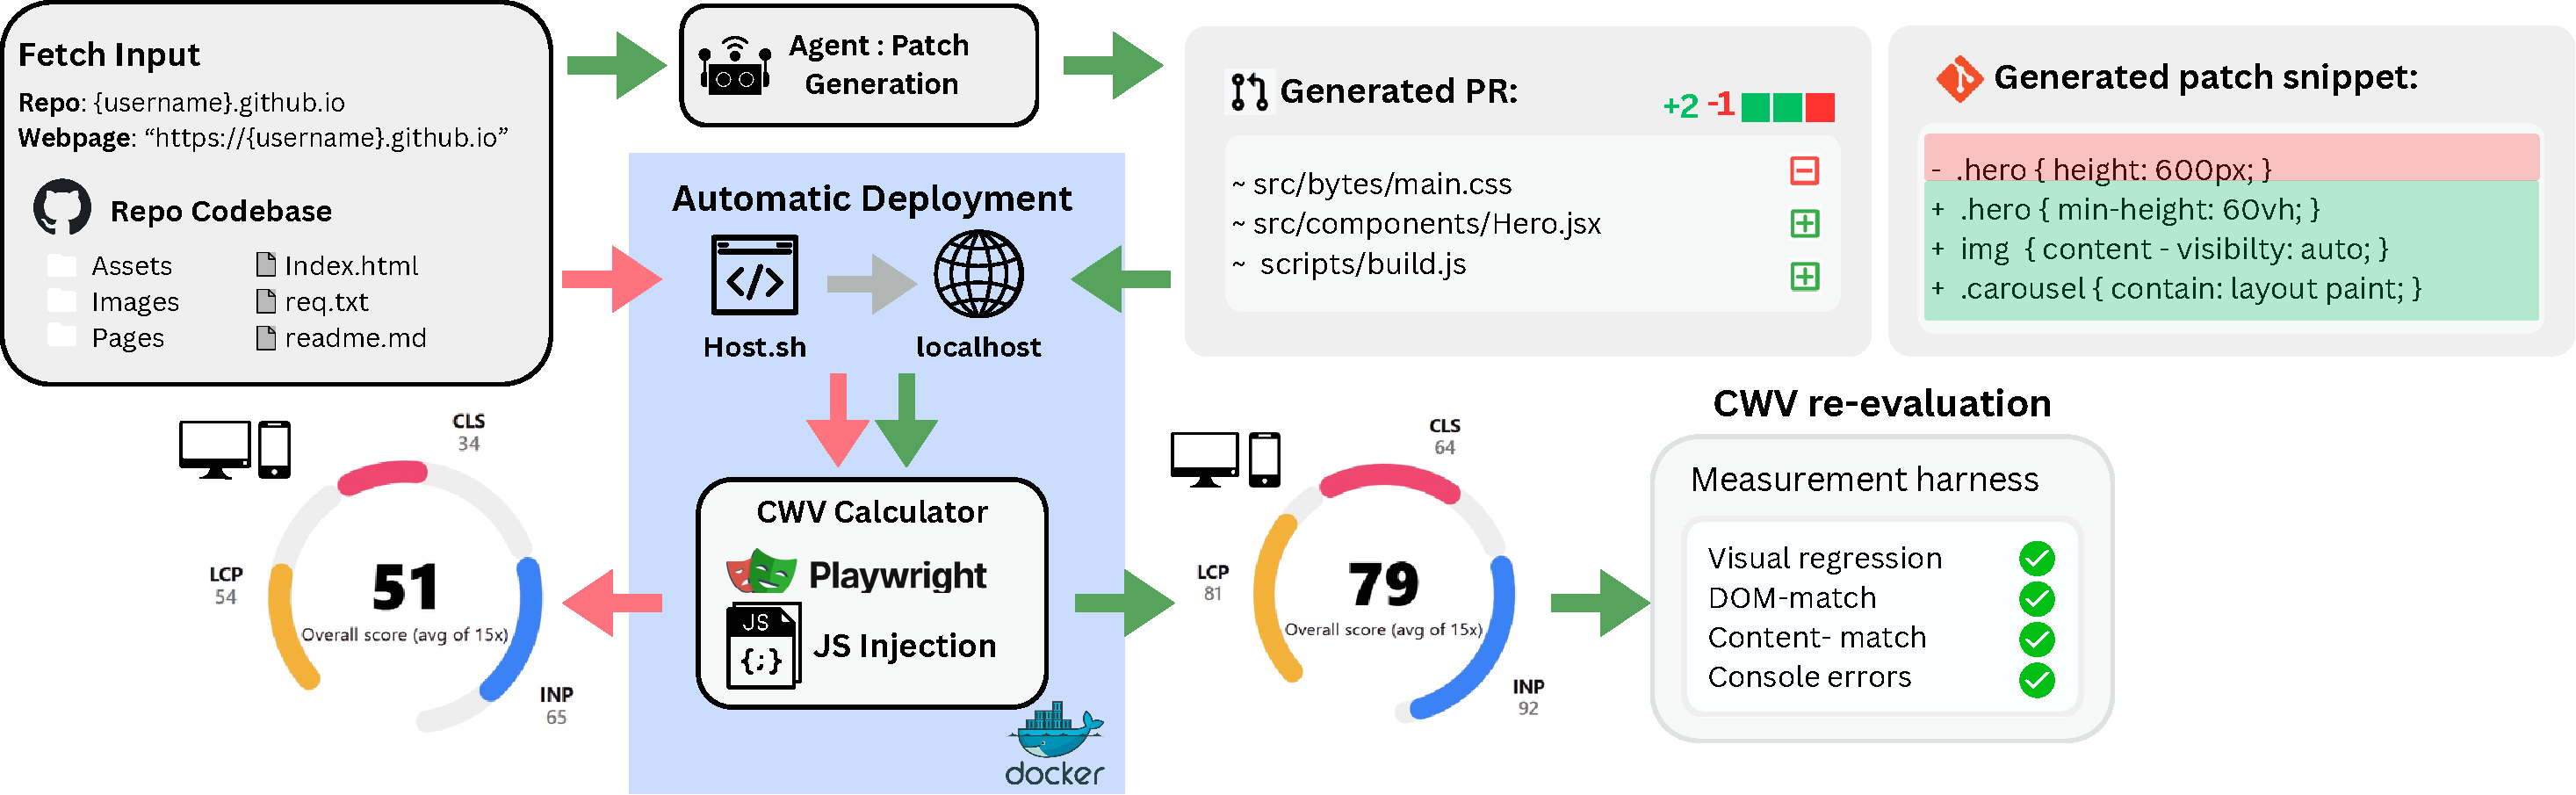
\includegraphics[width=\textwidth]{figures/Initial_Workflow.pdf}
  \caption{CWV Evaluation Harness: For each task, the harness fetches a pinned repository snapshot and deploys it locally via a deterministic host script. An agent generates a patch over the repository, after which the site is redeployed and re-evaluated. CWVs are computed via Playwright with injected Web Vitals instrumentation and repeated runs. Candidate patches must pass regression checks before improvements are scored.}
  \Description{A workflow diagram showing the CWV evaluation harness. A pinned repository snapshot is deployed locally, evaluated for baseline CWV metrics, modified by an agent, redeployed, and evaluated again with regression checks before the final score is computed.}
  \label{fig:evaluation_harness}
\end{figure*}

Large language models (LLMs) have progressed from code completion systems to autonomous software engineering agents. In parallel, evaluation paradigms have evolved from function-level synthesis \citep{austin2021programsynthesislargelanguage,chen2021codex} to repository-level issue resolution \cite{jimenez2024swebenchlanguagemodelsresolve}. Today's autonomous coding agents, exemplified by commercial tools such as Cursor\footnote{\url{https://cursor.com/}} and Claude Code\footnote{\url{https://claude.com/product/claude-code}}, can plan, use tools, and iteratively operate over entire codebases, and are already used or in planning by over 84\% of developers\footnote{\url{https://survey.stackoverflow.co/2025/}}. As these agents are increasingly deployed in real development workflows, the question of \emph{how to evaluate their true capabilities and real-world impact} has emerged as a central and unresolved challenge. While benchmark performance continues to improve \citep{openai_gpt5_3_codex_system_card_2026,anthropic_claude_opus_4_6_system_card_2026}, there is growing concern that existing evaluations fail to predict downstream impact, overestimate progress due to contamination, and don't capture the long horizon, goal directed behaviors that characterize practical software engineering.

Recent frontier research has begun to acknowledge this gap by arguing that meaningful evaluations should reflect real-world and economic outcomes. 
OpenAI introduced SWE-Lancer \citep{miserendino2025swe}, a benchmark comprising 1,400 real freelance software engineering tasks sourced from Upwork and collectively valued at over \$1M. Despite strong performance on existing benchmarks, frontier agents achieve low success rates on SWE-Lancer, highlighting a substantial gap between benchmark proficiency and economically meaningful software engineering capability. While SWE-Lancer demonstrates that outcome-based evaluation is both feasible and informative, achieving this required end-to-end tests triple-verified by more than a hundred experienced software engineers and additional manual validation by hiring managers. Such requirements make these evaluations slow, costly, and difficult to scale or continuously evolve. As a result, the community has largely relied on automated and reproducible benchmarks, with SWE-Bench Verified emerging as the most widely adopted across both open \citep{yang2025qwen3,zai_glm47_2025,team2025kimi} and closed-source models \citep{anthropic_claude_opus_4_6_system_card_2026,openai_gpt5_3_codex_system_card_2026,googledeepmind_gemini_models}. These benchmarks evaluate agents by their ability to fix issues sourced and manually filtered from public GitHub repositories against predefined test cases.

However, the community has increasingly recognized data contamination as a first-order challenge for such benchmarks \cite{deng2025swe}. Because modern models are trained on vast corpora of public code, static benchmarks constructed from public repositories risk measuring memorization rather than generalization. This limitation has become increasingly evident: SWE-Bench Pro reports that top models achieve only $\sim$23\% accuracy when evaluated on repositories and bugs sourced from private and licensed code, compared to 70\%+ on SWE-Bench Verified. This indicates that performance on public benchmarks can substantially overestimate real-world software engineering capability.

Even if contamination were fully mitigated, existing benchmarks like SWE-Bench and SWE-Bench Verified would still fail to capture a second critical dimension of real-world software engineering: goal-directed, long-horizon autonomy. Real development rarely consists of isolated, single-patch fixes, instead, it involves interpreting high-level objectives, diagnosing complex systems, coordinating multi-file changes, iterating based on feedback, and preserving existing functionality over time. Recent work such as SWE-EVO \cite{thai2025swe} highlights that current benchmarks inadequately elicit such behaviors, revealing a substantial gap between agents' performance on short-horizon issue fixing and their ability to carry out sustained, goal-driven development. Further, existing repository-level benchmarks such as SWE-Bench and its derivatives consist of Python Repositories only, despite JavaScript and TypeScript being the most prevalent languages ($>$40\%) on GitHub and dominating modern web development workloads\footnote{\url{https://github.blog/news-insights/octoverse/}}

Taken together, these frontier efforts establish three crucial requirements for next generation coding agent evaluation: (i) \textbf{alignment with real-world impact}, (ii) \textbf{resistance to data contamination}, and (iii) \textbf{support for open-ended, long-horizon, goal-directed autonomy}. Existing benchmarks satisfy at most one or two of these criteria, leaving a critical gap in our ability to meaningfully assess autonomous software engineering agents. In this work, we introduce \OurBench, an execution-based continuous optimization benchmark designed to fill this gap by evaluating coding agents on their ability to improve real websites' user-facing performance. Rather than measuring correctness against predefined test cases, \OurBench tasks agents with optimizing Core Web Vitals (CWVs; see \ref{sec:background_cwv}), which capture loading speed, responsiveness, and visual stability as experienced by end users on deployed webpages. Each webpage constitutes a task: agents are given access to the full source repository and may freely modify the codebase to improve measured performance. Success is defined by consistent improvement in CWVs relative to a baseline, rather than matching a reference patch. We provide an open-source, dockerized, fully automated execution harness that enables reproducible evaluation.

CWVs provide a strong proxy for real-world and economic impact. Improvements in CWVs are tightly correlated with downstream engagement metrics such as bounce rate, session duration, and conversion, which directly drive traffic retention, revenue, and long-term search visibility with industrial reports\footnote{\url{https://www.deloitte.com/ie/en/services/consulting/research/milliseconds-make-millions.html}} demonstrating that just a 0.1s improvement in LCP increased conversions and order values by upto 10\%, positioning CWVs as an impact-aligned reward signal. Crucially, \OurBench does not depend on manual reference solutions or static test cases that models could memorize. Even if models have been trained on the underlying source repositories, they cannot directly memorize the evaluation target, since Core Web Vitals are measured dynamically from deployed webpages rather than matched against reference patches reducing the scope of contamination. Moreover, the benchmark can continuously refresh as new repositories are added, further mitigating contamination and saturation over time. As developers keep adding new features and webpages, it requires continuous optimization. 

Beyond contamination resistance, web performance optimization is inherently
open-ended and goal-directed, making it a natural probe for long-horizon
autonomy. A single webpage may expose multiple interacting bottlenecks: slow
resource loading, render-blocking scripts, layout instability, admitting
many valid improvement strategies and require coordinated changes across
assets, configuration, and application logic. Crucially, optimizing one
metric (e.g., Largest Contentful Paint) can silently degrade another (e.g.,
Cumulative Layout Shift), demanding that agents not only improve performance
but also avoid collateral regressions across the full metric surface. This
multi-objective structure, combined with the need for iterative diagnosis,
planning, and tool-mediated code editing, naturally elicits the kind of
sustained, goal-driven reasoning that short-horizon benchmarks leave
untested.

Using \OurBench, we evaluate four modern coding agents paired with four
frontier LLMs on 300 websites. Our results expose a striking capability gap:
even the best configuration (OpenCode + GPT-5.1\,Codex) improves CWVs without
regressions on only 57\% of sites, while weaker models degrade
more sites than they help, with up to 90\% degradation rates. Notably, even
with appropriate scaffolding, full tool access vanilla prompting with any model and agent yields a 0\% improvement rate, and improvements are only seen when agents are provided with a custom structured plan-then-implement protocol. Controlled ablations reveal that the agent scaffold
and the underlying LLM contribute in complementary ways: the scaffold
governs multi-metric planning (a 16$\times$ improvement across agents), while the weaker models cause regressions. These findings position CWV optimization as a frontier challenge for autonomous coding agents and demonstrate the value of impact-aligned, execution-based evaluation. We highlight the following contributions:

\begin{enumerate}
    \item We introduce SWE-Experience-Bench, the first execution-based benchmark that evaluates autonomous coding agents on improving user-facing performance metrics (Core Web Vitals) for real, deployed websites, live GitHub Pages sites verified against their public renderings spanning 2{,}741 repositories and 73{,}000 deduplicated webpages across 11 popular web frameworks (including React, Vue, Next.js, Hugo, and Jekyll) that collectively cover 70\% of the most widely used web stacks on GitHub Pages.
    \item We design a framework-agnostic, containerized evaluation harness that automatically deploys websites, measures CWVs under controlled conditions, and ensures there are no visual regressions, build errors, or content addition/removal in the updated webpage, ensuring the agent cannot hack the evaluation by removing content or functionalities.
    \item We present a scalable benchmark curation and refresh pipeline that mitigates data contamination and saturation by continuously incorporating new repositories and technology stacks. This makes the benchmark reusable for rapidly improving LLMs and Software Engineering Agents.
    \item We conduct a systematic evaluation of four coding agents paired with four frontier LLMs, revealing substantial gaps between short-horizon bug fixing and long-horizon performance optimization. We observe improvements in Core Web Vitals (CWVs) on up to 57\% of websites, with GPT-5.1-Codex emerging as the most successful LLM and OpenCode as the most effective agent. These agents can also improve websites beyond Google Lighthouse’s ``Good" certification threshold. Controlled ablation studies demonstrate the importance of both agent scaffolding and the underlying LLM. However, models remain poor at improving CLS and INP metrics, and at autonomously leveraging scaffolding when using vanilla prompting.
\end{enumerate}



 % \item We conduct a systematic evaluation of modern coding agents, revealing substantial gaps between short-horizon bug fixing and long-horizon performance optimization, \arnav{across various state-of-the-art LLMs}. \somesh{add a few more lines about key results - are we able to increase CWV across the board - good and bad websites? which llms are best? how much time do they take? would throwing more budget solve the problem? is there some scaling law? are LLMs exploring enough? when do they give up? what is the path forward?}